% This is a simple template for a LaTeX document using the "article" class.
% See "book", "report", "letter" for other types of document.

\documentclass[fleqn, hidelinks]{article} % use larger type; default would be 10pt

\usepackage[utf8]{inputenc} % set input encoding (not needed with XeLaTeX)

%%% Examples of Article customizations
% These packages are optional, depending whether you want the features they provide.
% See the LaTeX Companion or other references for full information.

%%% PAGE DIMENSIONS
\usepackage{geometry} % to change the page dimensions
\geometry{a4paper} % or letterpaper (US) or a5paper or....
% \geometry{margin=2in} % for example, change the margins to 2 inches all round
% \geometry{landscape} % set up the page for landscape
% read geometry.pdf for detailed page layout information

\usepackage{graphicx} % support the \includegraphics command and options

\usepackage[parfill]{parskip} % Activate to begin paragraphs with an empty line rather than an indent

\usepackage[none]{hyphenat}

%%% PACKAGES
\usepackage{booktabs}
\usepackage{array}
\usepackage{paralist}
\usepackage{fancyvrb}
\usepackage{cite}
\usepackage{url}
\usepackage{amsmath}
\usepackage{enumitem} %some fancy list stuff
\usepackage{caption}
\usepackage{subcaption}
\usepackage[english]{babel}
\usepackage{float}

%%% HEADERS & FOOTERS
\usepackage{fancyhdr} % This should be set AFTER setting up the page geometry
\pagestyle{fancy} % options: empty , plain , fancy
\raggedright
\renewcommand{\headrulewidth}{0pt} % customise the layout...
\lhead{}\chead{}\rhead{}
\lfoot{}\cfoot{\thepage}\rfoot{}

%%% SECTION TITLE APPEARANCE
%\usepackage{sectsty}
%\allsectionsfont{\sffamily\mdseries\upshape} % (See the fntguide.pdf for font help)
% (This matches ConTeXt defaults)

%%% ToC (table of contents) APPEARANCE
\usepackage[nottoc,notlof,notlot]{tocbibind} % Put the bibliography in the ToC
\usepackage[titles,subfigure]{tocloft} % Alter the style of the Table of Contents
\renewcommand{\cftsecfont}{\rmfamily\mdseries\upshape}
\renewcommand{\cftsecpagefont}{\rmfamily\mdseries\upshape} % No bold!

\newcommand{\CO}{\textsc{co}$_2$~}
\newcommand{\mtext}[1] {\text{\emph{#1}}}

%%% A couple of commands for the title page
\usepackage{hyperref}
\newcommand{\HRule}{\rule{\linewidth}{0.5mm}}

%%% END Article customisations

%%% The "real" document content comes below...
\author{Nikunj Patel (np1509) \& Farhan Rahman (fr909)}
\title{Advanced Computer Graphics Coursework}
\date{\today}
%\date{} % Activate to display a given date or no date (if empty),
% otherwise the current date is printed 

\begin{document}
\maketitle
\section{Part1: Generate plots of Fresnel Reflectance}

In this part, the task was to generate the reflectance behaviour for dielectric materials. The fresnel reflectance for parallel and perpendicular polarised light can be formulated as follows in equations \ref{eqn:rparallel} and \ref{eqn:rperpendicular} respectively.

\begin{equation}
	r_{||} = {\left|\frac{\eta_{i} cos(\theta_{t}) - \eta_{t} cos(\theta_{i})}{\eta_{i} cos(\theta_{t}) + \eta_{t} cos(\theta_{i})} \right|}^2
	\label{eqn:rparallel}
\end{equation}

\begin{equation}
	r_{\perp} = {\left|\frac{\eta_{i} cos(\theta_{i}) - \eta_{t} cos(\theta_{t})}{\eta_{i} cos(\theta_{i}) + \eta_{t} cos(\theta_{t})}\right|}^2
	\label{eqn:rperpendicular}
\end{equation}

The Fresnel reflectance behaviour for parallel and perpendicular polarized components was generated for light entering a medium having an index of refraction ($\eta_{t}$) = 1.5. Similarly the reflectance was generated for light exiting the medium into air, which has an index of refraction of 1.0. Figure \ref{fig:enter} shows the Fresnel Reflectance behaviour for light entering the medium. 

{\bf Light entering medium:}

Reflectance at 0 degrees (\%): 4 \\
Brewster's angle (degrees): 56 \\
Reflectance at Brewster's angle (\%): 0.00104423

Figure \ref{fig:exit} shows the reflectance behaviour for light exiting the medium and entering air.

{\bf Light exiting medium:}

Reflectance at 0 degrees (\%): 4 \\
Brewster's angle (degrees): 34 \\
Reflectance at Brewster's angle (\%): 0.005635 \\
Critical angle (degrees): 41

\begin{figure}
	\centering
	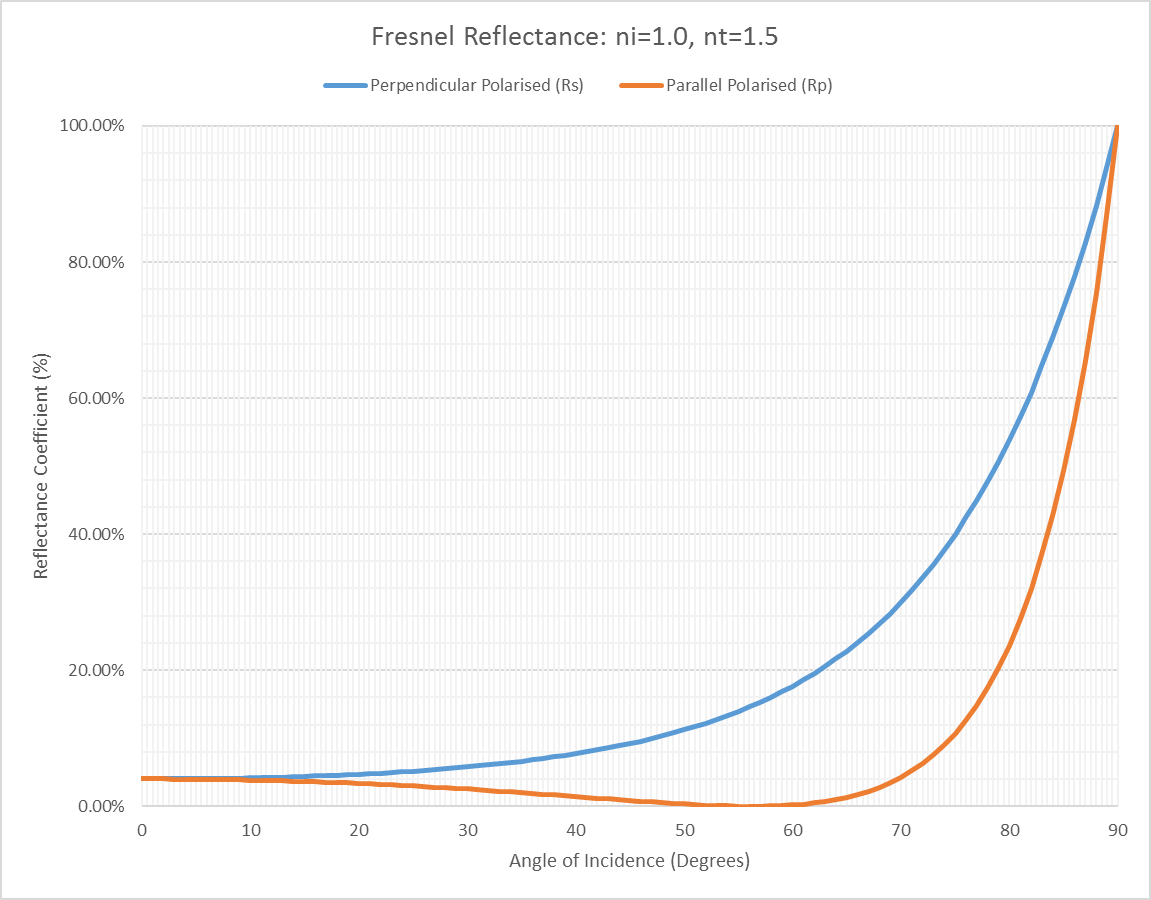
\includegraphics[width=\textwidth]{imgs/enter1.png}
	\caption{Fresnel Reflectance for light entering medium $\eta_{i} = 1.0$, $\eta_{t} = 1.5$}
	\label{fig:enter}
\end{figure}

\begin{figure}
	\centering
	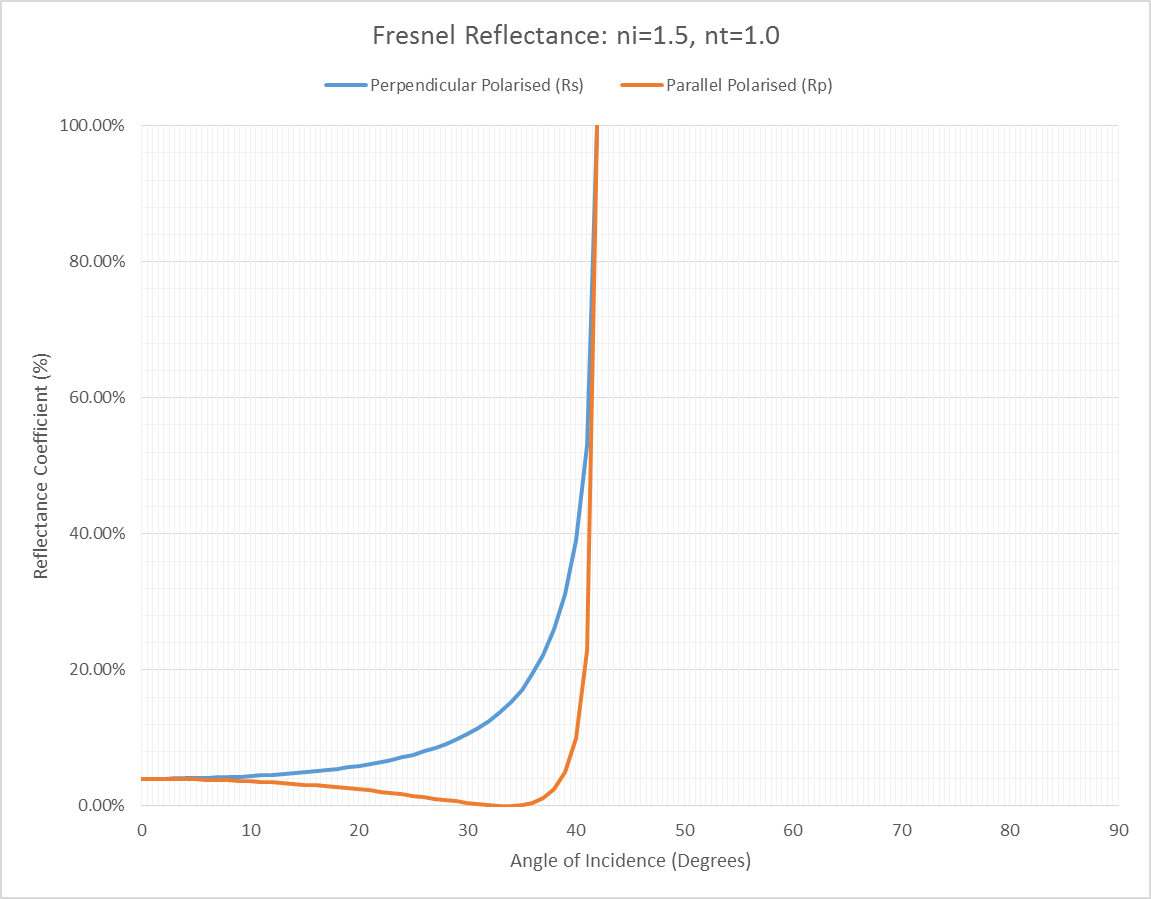
\includegraphics[width=\textwidth]{imgs/exit1.png}
	\caption{Fresnel Reflectance for light exiting medium $\eta_{i} = 1.5$, $\eta_{t} = 1.0$}
	\label{fig:exit}
\end{figure}


\section{Part2: Generate samples according to an Environment Map}

The 2D cumulative distribution functions were generated first. These were the P(X) generated from the average energy per column and P(Y) which is the cumulative distribution function for every column or scan line. Each average or luminance value of a pixel was scaled by the sine of it's relative theta position in the Latitude-Longitude space. The samples were generated by first sampling along the columns and then sample along the rows for that particular column. Once the sample was obtained, a 5x5 grid was used to set the pixel value in the image to green. This process was done for 64, 256 and 1024 samples. Figure \ref{fig:EMSampling} shows the results.

\begin{figure}
        \centering
        \begin{subfigure}[b]{\textwidth}
                \centering
                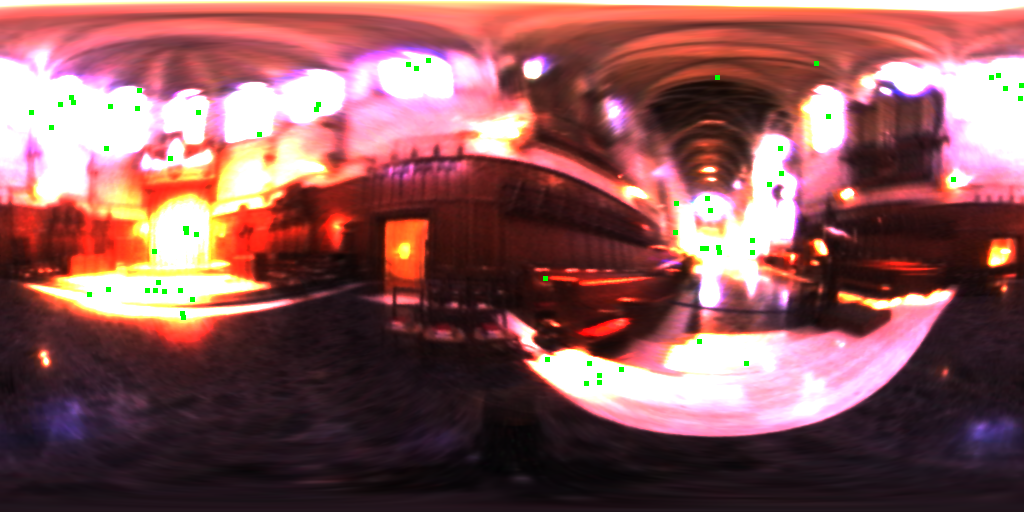
\includegraphics[width=0.7\textwidth]{imgs/Part2/env64.png}
                \caption{}
                \label{fig:env64}
        \end{subfigure}
        \begin{subfigure}[b]{\textwidth}
                \centering
                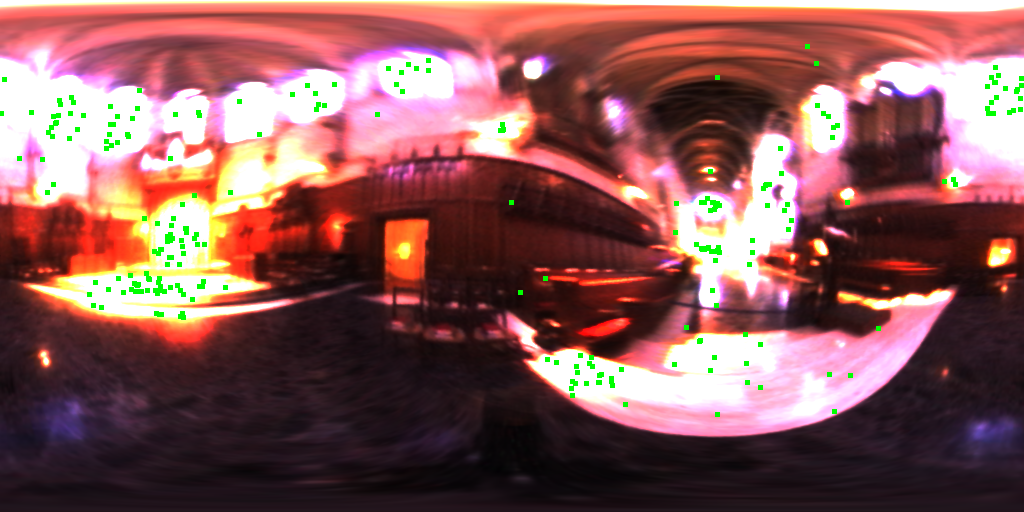
\includegraphics[width=0.7\textwidth]{imgs/Part2/env256.png}
                \caption{}
                \label{fig:env256}
        \end{subfigure}
        \begin{subfigure}[b]{\textwidth}
                \centering
                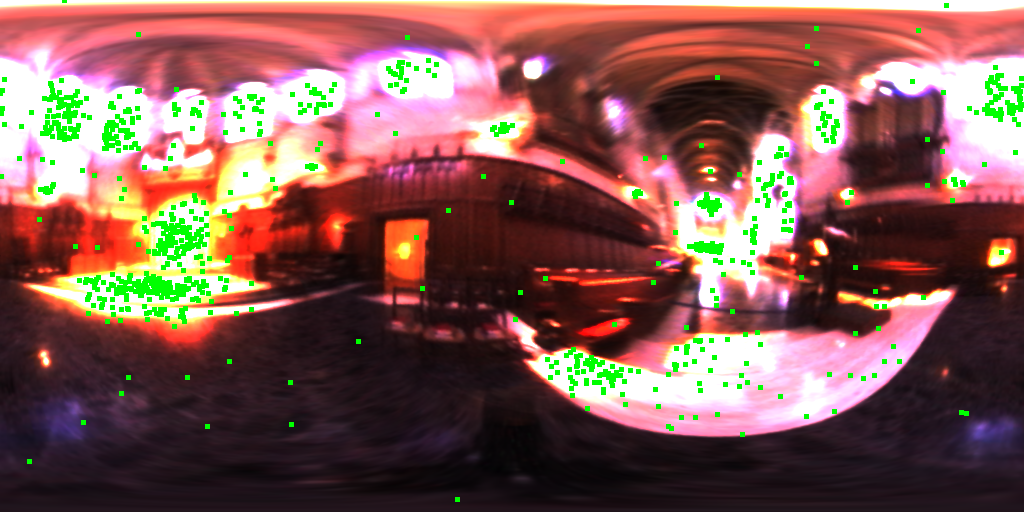
\includegraphics[width=0.7\textwidth]{imgs/Part2/env1024.png}
                \caption{}
                \label{fig:env1024}
        \end{subfigure}
        \caption{\ref{fig:env64}, \ref{fig:env256} and \ref{fig:env1024} shows environment map sampled with 64, 256 and 1024 samples respectively}\label{fig:EMSampling}
\end{figure}


\section{Part3: Generate samples according to Phong BRDF}

In this part the environment map was sampled according to the Phong BRDF model. The Phong BRDF model can be parameterised as follows:

\begin{equation}
	(\theta, \phi) = (arcos((1-\mu_1)^{\frac{1}{n+1}}), 2\pi\mu_2)
	\label{eqn:phong}
\end{equation}

The phong lobe was then sampled with exponents 1.0, 10.0, 50.0 and 200.0. The results of these are shown in Figure \ref{fig:PhongSampling}.

\begin{figure}
        \centering
        \begin{subfigure}[b]{\textwidth}
                \centering
                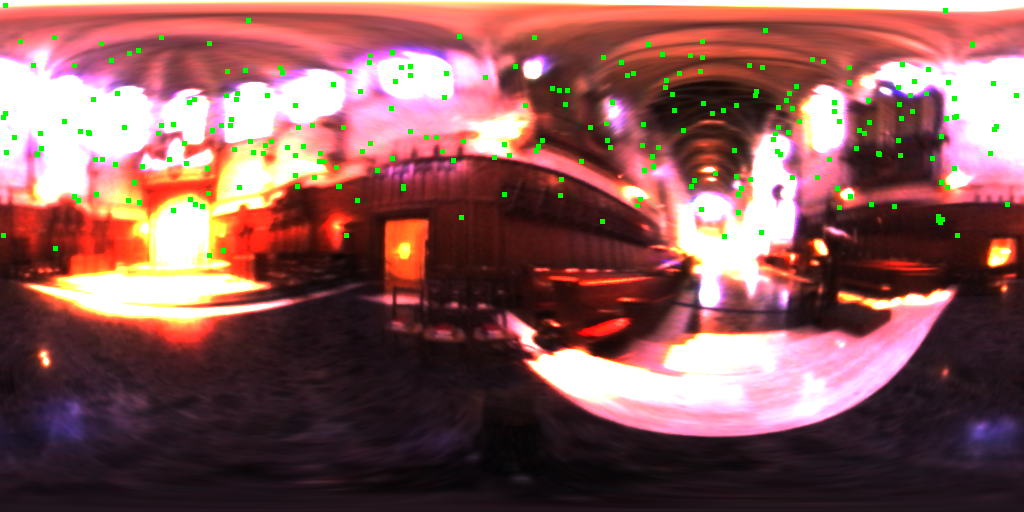
\includegraphics[width=0.6\textwidth]{imgs/Part3/env1.png}
                \caption{}
                \label{fig:env1}
        \end{subfigure}
        \begin{subfigure}[b]{\textwidth}
                \centering
                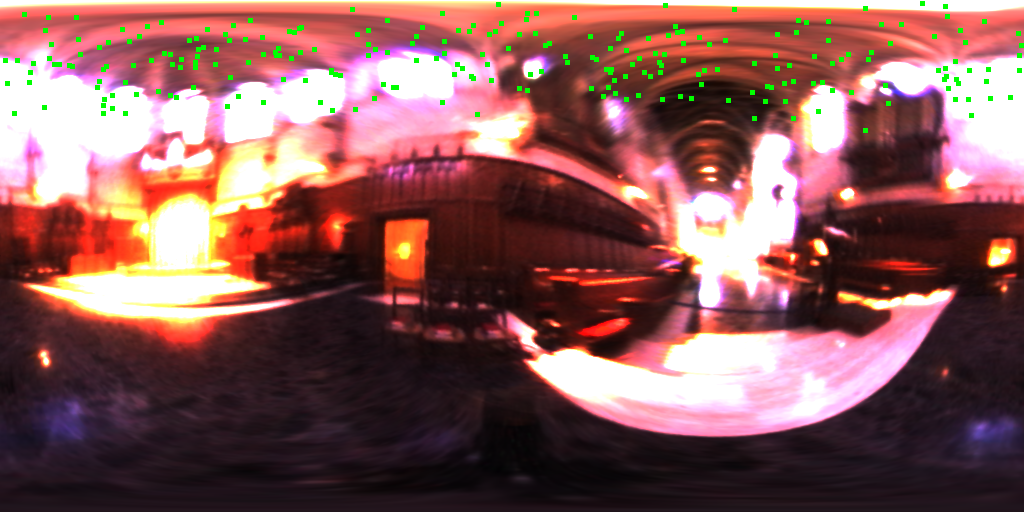
\includegraphics[width=0.6\textwidth]{imgs/Part3/env10.png}
                \caption{}
                \label{fig:env10}
        \end{subfigure}
        \begin{subfigure}[b]{\textwidth}
                \centering
                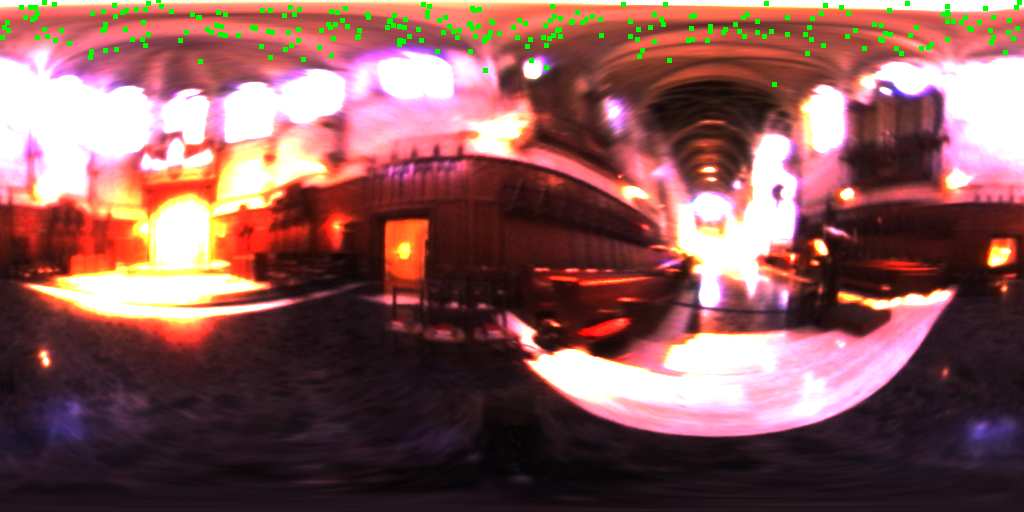
\includegraphics[width=0.6\textwidth]{imgs/Part3/env50.png}
                \caption{}
                \label{fig:env50}
        \end{subfigure}
        \begin{subfigure}[b]{\textwidth}
                \centering
                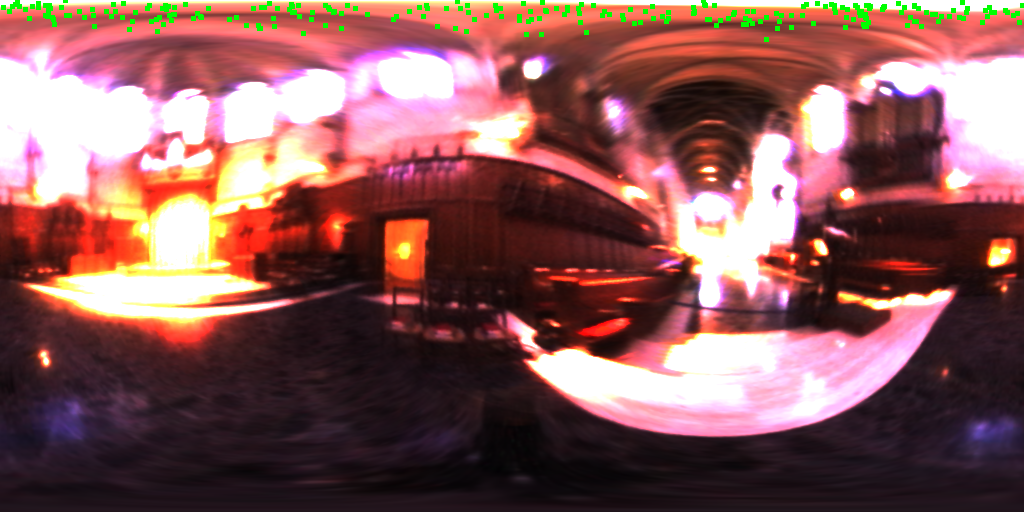
\includegraphics[width=0.6\textwidth]{imgs/Part3/env200.png}
                \caption{}
                \label{fig:env200}
        \end{subfigure}        
        \caption{\ref{fig:env1}, \ref{fig:env10}, \ref{fig:env50} and \ref{fig:env200} shows environment map sampled with phong exponents 1.0, 10.0, 50.0 and 200.0 respectively}\label{fig:PhongSampling}
\end{figure}


\section{Part4: Render a sphere with sampled Environment Map}

Figure \ref{fig:Part4} shows the results of sampling a sphere from the environment maps using different number of samples.

\begin{figure}
        \centering
        \begin{subfigure}[b]{\textwidth}
                \centering
                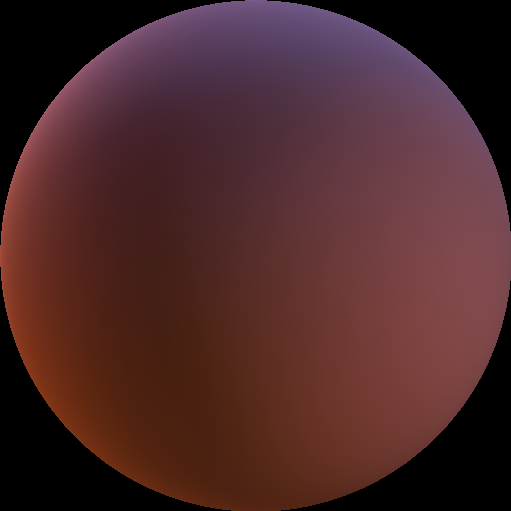
\includegraphics[width=0.4\textwidth]{imgs/Part4/sphere64.png}
                \caption{}
                \label{fig:sphere64}
        \end{subfigure}
        \begin{subfigure}[b]{\textwidth}
                \centering
                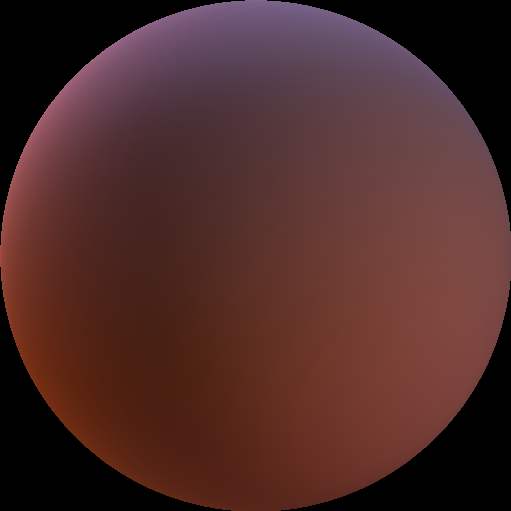
\includegraphics[width=0.4\textwidth]{imgs/Part4/sphere256.png}
                \caption{}
                \label{fig:sphere256}
        \end{subfigure}
        \begin{subfigure}[b]{\textwidth}
                \centering
                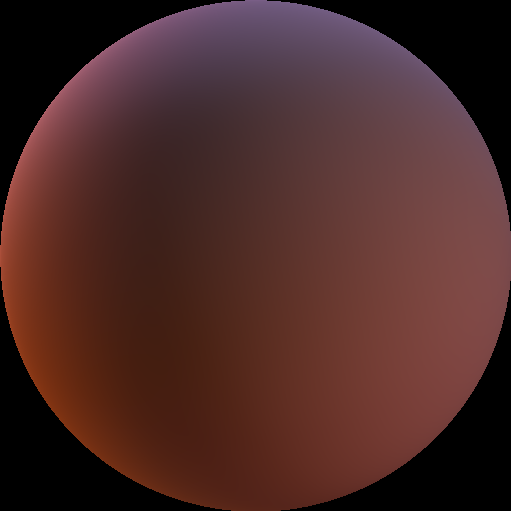
\includegraphics[width=0.4\textwidth]{imgs/Part4/sphere1024.png}
                \caption{}
                \label{fig:sphere1024}
        \end{subfigure}
        \caption{\ref{fig:sphere64}, \ref{fig:sphere256} and \ref{fig:sphere1024} shows diffuse spheres sampled from the environment map with 64, 256 and 1024 samples respectively}\label{fig:Part4}
\end{figure}

\end{document}